% !TeX document-id = {04156f11-6e1c-4c0d-8b85-6e701dbcf684}
%% The first command in your LaTeX source must be the \documentclass command.
%%
%% Options:
%% twocolumn : Two column layout.
%% hf: enable header and footer.
\documentclass[
% twocolumn,
% hf,
]{ceurart}
%
\usepackage{makeidx}  % allows for indexgeneration
%\usepackage[pdftex]{graphicx}
\usepackage[T1]{fontenc}
\usepackage[utf8]{inputenc}
\usepackage{upquote}
%
\begin{document}

%%
%% Rights management information.
%% CC-BY is default license.
\copyrightyear{2021}
\copyrightclause{Copyright for this paper by its authors.
	Use permitted under Creative Commons License Attribution 4.0
	International (CC BY 4.0).}

%%
%% This command is for the conference information
\conference{OCL 2021: 20th International Workshop on OCL and Textual Modeling, June, 2021, Bergen, Norway}

%%
%% The "title" command
\title{A Validity Analysis to Reify 2-valued Boolean Constraints}

%%
%% The "author" command and its associated commands are used to define
%% the authors and their affiliations.
\author[1]{Edward D. Willink}[%
email=ed at willink.me.uk,
]
\address[1]{Willink Transformations Ltd, Reading, England}

%%
%% The abstract is a short summary of the work to be presented in the
%% article.
\begin{abstract}
As an executable specification language, OCL enables metamodel constraints that cannot be sensibly expressed graphically to be resolved textually. However many users have expressed disquiet that although a constraint is obviously either satisfied or not, the OCL formulation is not 2-valued. We argue that this disquiet is the consequence of a misunderstanding emanating from the failure of the OCL specification to address crashing. We introduce an analysis that identifies potentially invalid computations and so guarantees that Constraints are 2-valued and that OCL-based Model Transformations do not malfunction.
\end{abstract}

%%
%% Keywords. The author(s) should pick words that accurately describe
%% the work being presented. Separate the keywords with commas.
\begin{keywords}
  Program Validation \sep
Model Transformation \sep
OCL \sep
Crash
\end{keywords}

%%
%% This command processes the author and affiliation and title
%% information and builds the first part of the formatted document.
\maketitle

\section{Introduction}
%
OCL \cite{OCL-2.4} evolved from Syntropy to satisfy the need to elaborate UML \cite{UML-2.5} diagrams with constraint details that could not sensibly be expressed graphically. Within the context of a UML model, OCL specifies what happens within a domain-specific Utopia where nothing bad happens, not even when the user models real problems.

OCL is a specification language that is also executable and so the OCL specification makes concessions to realizability by prohibiting infinite collections such as \verb|Integer.allInstances()| and tolerating indeterminacy for operations such as \verb|Set::asOrderedSet()|. However there is no concession to 32 bit integers or floating point precision. These details pale in comparison to the major oversight of what happens when things go wrong.

In this paper we review the ways in  which OCL can go wrong and introduce a validity analysis so that we can guarantee that OCL will always crash desirably and never crash undesirably.

We use the emotive term crash for the problem since all programmers understand what a crash is. It avoids any confusion with solutions where terms such as invalid/exception/error/failure are used.

In Section~\ref{Crashes} we review the ways in which OCL can crash so that in Section~\ref{Goal} we outline what we need to achieve and in what respects the OCL specification needs to be tweaked. Section~\ref{Running Example} presents a running example to show how even the simplest of invariants may be unsafe. In Section~\ref{Program Analysis} we introduce the analysis and symbolic evaluation that diagnoses all crash hazards and in Section~\ref{Corollaries} we identify opportunities for better practice that exploits the validity analysis. In Section~\ref{Current Status and Further Work} we describe how far the implementation work has progressed.  Finally in Section~\ref{Related Work} we review the related work and conclude in Section~\ref{Conclusions}.

\section{Crashes}\label{Crashes}

Programmers in most languages are resigned to the need to debug their programs to fix bugs and to handle exceptions where problems are unavoidable. OCL has no exception capability. Rather than throwing an exception as an out-of-band `return', OCL returns the \verb|invalid| singleton value as an in-band result. In principle, these two mechanisms are equivalent, particularly if a practical OCL implementation supports a richer \verb|invalid| that includes details of the problem while continuing to behave as a singleton.

Many OCL programmers are unhappy that the in-band return of \verb|invalid| means that an OCL Constraint is not 2-valued despite being a self-evident arbiter of whether some condition is satisfied or not. This unhappiness is actually a misunderstanding \cite{OCLreflections} since any non-trivial constraint expressed in almost any language has three possible outcomes; satisfied, not-satisfied and crash. The misunderstanding arises because, when the crash uses an exception mechanism, the crash outcome bypasses the invocation code, which perceives only two outcomes. In contrast, the OCL programmer must ensure that the invocation propagates the \verb|invalid| back to the invocation's caller. The misunderstanding is therefore an ergonomic issue whereby the API provided by the OCL evaluator fails to meet the expectations of the user and fails to alert the programmer to the simple solution of converting an OCL \verb|invalid| result into an exception to propagate the crash.

It would clearly be better if programs do not crash, but before we look at reasons for OCL to crash, we will look at mechanisms that avoid some crashes.

\subsection{Crash Avoidance}

\subsubsection{Well Formedness Rules} OCL expression terms such as \emph{PropertyCallExp} navigate a model in accordance with its metamodel, which provides a strong type system with which the OCL expressions must comply. Compliance is defined by the Well Formedness Rules that can check that for instance the type of the \emph{ownedSource} of a \emph{PropertyCallExp} conforms to the \emph{owningClass} of its \emph{referredProperty}.

An OCL validator should check all the WFRs, preferably at edit time, but at least before execution, since execution is likely to fail miserably if a WFR is violated. We may therefore assume that no crash occurs as a consequence of a WFR violation.

\subsubsection{Guards}\label{Guards} Where a programmer is aware that a crash may occur, the programmer may guard against it. A substantive guard may use an \verb|if then else endif| to provide alternative functionality, or a more localized guard may use a logical operator.

\begin{verbatim}
    (var != null) || var.doSomething()		// C or Java
\end{verbatim}

The Java above uses the short-circuit \verb&||& operator to prevent a \emph{NullPointerException} when \verb|doSomething()| is invoked when \verb|var| is \verb|null|.

As we shall see, the equivalent OCL operator is not short-circuit. Rather than preventing a crash, it can allow a crash to happen and then require the crash to be uncrashed.

\subsection{Catastrophic / Desirable Crashes}

Problems such as Power Failure, Stack Overflow or Memory Allocation Failure can occur at almost any time and there is nothing that a normal OCL program can do about them.

Problems such File Access, Network or Database failure may occur when a \emph{NavigationCallExp} requires an additional model element to be available. Again there is very little that a normal OCL program can do about them.

These problems are pretty catastrophic. We categorize the consequent crashes as desirable since the most sensible response is to diagnose the problem as helpfully as possible in the hope that the user may understand and resolve the issue.




%An OCL execution results from the collaboration of the execution of each OCL Abstract Syntax Tree element. We must therefore examine each AST element for crash hazards, very few of which are mentioned in the OCL specification.

%Purely declarative elements such as \emph{IntegerLiteralExp| or \emph{Property| or \emph{Variable| involve no execution, however depending on implementation subtleties, it may be while preparing to support the declaration that a generally catastrophic Power Failure, Stack Overflow or Memory Allocation Failure occurs.

%Simple execution elements such \emph{IfExp| or \emph{LetExp| or \emph{VariableExp| use only facilities that are likely to be in registers or on the stack and so are again only subject to catastrophic failures.

%An \verb|IteratorExp| or \verb|OperationCallExp| is much more vulnerable to a Stack Overflow from an imprudent recursion or to a type failure for an unsuitable source or argument input. 

%An \verb|NavigationCallExp| is vulnerable to a File Access, Network or Database failure when the accessed Property is provided by an out-of-memory source.


%Most of the foregoing failures are catastrophic and the OCL language provides no mechanism to avoid the crash. For normal applications there is little than can be done. We therefore categorize these as desirable crashes since they should propagate to an outer invocation environment that provides as much helpful diagnosis to the user as possible.

%The exception to this observation is that a null navigation is the result of defective programming and so we categorize it as an undesirable crash that the programmer should avoid.

%While some Operating System level programs may react to certain crashes by retrying with more memory or on a different processor, for the vast majority of OCL programs the crash is desirable and we do not want to cover it up.

\subsection{Careless / Undesirable Crashes}

OCL supports a \verb|null| value to reify the content of slots with optional multiplicities and an \verb|invalid| value to reify the consequence of an evaluation failure. These values are not suitable for computation and so OCL defines a strict semantics whereby usage in \emph{IteratorExp}, \emph{OperationCallExp} or \emph{NavigationCallExp} is a failure that results in an \verb|invalid| value result.
The loose wording in the specification could be formalized by preconditions for the evaluation counterpart of the expression.

\begin{verbatim}
    context NavigationCallExpEval
    pre ValidSource: not source.oclIsInvalid();
    pre NonNullSource: not source.oclIsUndefined();
\end{verbatim}

Failure of a precondition is a consequence of careless programming, we therefore categorize it as an undesirable crash. The programmer needs assistance to ensure that such crashes never occur.

The strict execution semantics of the OCL Abstract Syntax Tree elements provides a simple crash-and-stay-crashed behavior. The OCL Standard Library defines

\begin{itemize}
	\item regular operations with preconditions
	\item irregular not-strict logical operations
	\item special operations that may use \verb|OclVoid| or \verb|OclInvalid| types
\end{itemize}

The additional preconditions provide further opportunities for careless programming.

%The OCL Standard Library also provides mechanisms to uncrash a crash so that we now have undesirable crashes whose crash may need to be suppressed.

\subsubsection{Divide-by-Zero}

The problem of divide-by-zero exists in many languages, but is relatively rare in practice and often easily avoided. OCL is little used for arithmetic, so the problem hardly exists in practical OCL, but it would nonetheless be nice to avoid the crash.

\subsubsection{Index-out-of-bounds}

The \verb|OrderedSet| and \verb|Sequence| collection types support indexing in much the same way as \verb|Array| and \verb|List| in other languages. A crash occurs when an unsuitable index access is used. This problem occurs more often than might be expected since many users accidentally use the 0-based index typical of an execution language, rather than the 1-based index of a specification.

\subsubsection{Missing Content}

The collection types support reverse indexing using the \verb|indexOf| operation or the \verb|any| iteration and crash when the indexing misses. The crash from \verb|indexOf| is excessive since a \verb|null| or negative return could signal the query miss less forcefully. It is unreasonable to expect every use of \verb|indexOf| to be guarded by an \verb|includes|.

\subsubsection{Bad String Content}

Operations such as \verb|String::toReal()| support the lexical conversion of a string to a more interesting type. They crash if the source string is incompatible with the conversion. This crash is again excessive since a \verb|null| could signal the conversion failure. It is impractical to expect the source string to always be lexically valid and completely pointless to require the user to write their own parser to be used in a guard.

\subsection{Uncrashing}

Once a crash has occurred, the programmer may take some action to handle it.

\subsubsection{Catching}

In many languages a crash is propagated by throwing an exception and subsequently catching it. In OCL, the crash is propagated as the \verb|invalid| value and may be `caught' by the \verb|OCLAny::oclIsInvalid()| operation.

\begin{verbatim}
    let result : OclAny = functionThatMayCrash() in
    if result.oclIsInvalid() then fixupCrash() else result endif
\end{verbatim}

Accommodating \verb|OCLAny::oclIsInvalid()| is inconvenient when realizing OCL by translation to a conventional language, since all usages of the conventional exception passing must convert to values wherever \verb|oclIsInvalid()| might be invoked.

Ideally the usage of \verb|oclIsInvalid()| would be limited to not-invalid preconditions and Operating System level OCL that really wants to catch a catastrophic failure to produce a friendly diagnostic or to perhaps retry on another computer.

\subsubsection{Reverting}

The avoidance of crashes by short-circuit operators in conventional languages was described in Section~\ref{Guards}. Unfortunately the equivalent logical operators in OCL were  specified to be commutative. The incompatibility between commutativity and short-circuiting was `resolved' by making the logical operators not-strict to allow them to handle \verb|null| or \verb|invalid|. The commutativity is mathematically elegant but the consequent 4-valued \{\verb|true|, \verb|false|, \verb|null|, \verb|invalid|\} Boolean is unpopular with users and has bad implementation consequences.

The conventional short-circuit suppresses the unwanted evaluation of the second term.

\begin{verbatim}
    (var != null) || var.doSomething()		// C or Java
\end{verbatim}

The hazardous second term is not evaluated; no crash occurs.

The OCL short-circuit is

\begin{verbatim}
    (var <> null) or var.doSomething()
\end{verbatim}

Since the operator is commutative an implementation has a free choice of the evaluation order, and may even use different processors to evaluate the two arguments concurrently. For less obvious OCL expressions, it may be unclear to user or tooling what the best evaluation order is. An implementation cannot in general avoid evaluating the `wrong' argument first before evaluation of the `right' argument provides the guard value and so requires the implementation to discard the `erroneous' crash.

Even if the implementation foregoes the concurrency opportunity and evaluates first argument first, the commutativity allows a programmer to accidentally specify the guard second, so the implementation must still support the uncrash. Of course no sensible programmer will program the guard term second so the implementation is just being forced to implement something that should never happen.

Except that it does. During development, it is not uncommon for the system or at least the OCL exposition to be defective. A user who has set a breakpoint in code associated with a crash may find the debugger stopping at the crash and be confused when that crash fails to propagate as expected. The problem is that  the crash during the first term evaluation may be inhibited by a malfunction in the second input evaluation. The overall execution may be pedantically correct, but at best CPU time has been wasted by crashing. More likely the developer spends significant time understanding the strange behavior possibly concluding, with some justification, that OCL execution is unreliable.
%Again, many languages support prevention of a crash by guarding the hazardous invocation. In OCL this idiom is supported by the logical operators.

%\begin{verbatim}
%	functionWillNotCrash() implies functionThatMayCrash()
%\end{verbatim}

%The extra \verb|functionWillNotCrash()| functionality predicts the hazard and returns \verb|false| when execution of \verb|functionThatMayCrash()| must be prevented.

Unfortunately the commutative not-strict logical operators break the simple crash-and-stay-crashed behavior.

%The violation of strictness by the logical operations causes significant implementation difficulties and, as we shall see, causes significant user difficulties as well. In conventional languages the guard idiom is supported by what is commonly referred to as short-circuit semantics so that after evaluation of just the first logical operator input the input value is examined to determine whether the second logical operator input is also evaluated. The first input guards and so inhibits a redundant and potentially very awkward second input evaluation. Operators such as \verb|&&| and \verb&||& are therefore not commutative.

%The OCL specification unfortunately retains the mathematical elegance of commutativity for \verb|and| and \verb|or| and so requires a problematic first term evaluation to be guarded by a second term evaluation. A practical OCL implementation, particularly one using multiple processors, cannot guarantee to determine the guard result before the crash. Consequently the intended guard mechanism is broken in so far as the crash cannot be prevented,rather the implementation must uncrash once the guard term evaluation is known.



%in much the same way as other languages and are in danger of crashing when an unsuitable index access is attempted. This problem occurs more often than might be expected since many users accidentally use the 0-based indexes typical of execution languages rather than the 1-based index of a specification language.



%Other problems such as
%\begin{itemize}
%	\item null navigation (NullPointerException in Java)
%	\item bad ordered collection index (IndexOutOfBoundsException) 
%	\item divide-by-zero (ArithmeticException)
%\end{itemize}
%are the consequence of defective programming. When they occur during evaluation of an OCL constraint, there is little that can be done to help the user. They are the reason why constraints cannot be 2-valued. It is not honest to misreport the undesirable failure as a constraint not-satisfied when the verdict of the constraint evaluation is unclear.

%Programmers have learned to use guards to avoid the undesirable crashes that they are aware of.

%In \cite{safe} null-safe navigation operator invariants and null-free Collections were introduced allowing many null navigation issues to be avoided, although in many cases the avoidance just moves the null-problem somewhere else.

%In this paper we outline a deeper analysis that can guarantee that all undesirable crashes are eliminated. In the same way that execution of type-unsafe OCL is prohibited by a validation tool that checks the Well Formedness Rules, the new validity analysis can prohibit undesirable crashes.

\subsection{Model Transformation}

Many model transformation tools provide a disciplined framework to create or mutate an output model using immutable OCL queries on the input model. OCL crashes pose a difficult problem.

Some transformation languages such as QVTo \cite{QVT-1.3} provide a relatively conventional exception mechanism allowing the users to handle OCL's \verb|invalid| as an exception. %This is perhaps the worst of both worlds.

For declarative transformations, functionality is modularized by rules within which OCL specifies the matches and conversions. Execution is determined by the successful rule matches, so potentially an OCL crash just loses a rule match and the user is disappointed that some conversion did not happen. This is dishonest. Any crash is a transformation execution failure and any subsequent result is a suspect compromise. A declarative model transformation must crash enthusiastically.

When interpreting or generating code for a model transformation, the implementation must faithfully realize all possible OCL failures so that no crash is hidden. This requires considerable effort to support a behavior whose result is going to be thrown away. Much better to alert the programmer to all the undesirable crashes so that only desirable crashes remain allowing for a much simpler execution in which any crash is a fatal crash.
 
%\subsection{Transitive}
 
%Operations such as  \verb|Sequence::first()| can crash since they are just a convenience wrapper for \verb|Sequence::at(1)|. Similarly iterations such as \verb|exists| and \verb|forAll| can crash as a consequence of their iteration over the logical \verb|or| / \verb|and| operations. An implementation iterating over the non-strict logical operations must be prepared to crash many times before encountering a guard that inhibits the many crashes.
 
\section{Goal}\label{Goal}

We have motivated our goal for normal OCL
\begin{itemize}
	\item catastrophic/desirable crashes always crash
	\item careless/undesirable crashes never occur
\end{itemize}

This is fully in accord with OCL's strict behavior provided preconditions are always satisfied. We need a validity analysis that can guarantee this proviso.

The not-strict commutative specification of the logical operators conflicts with both our goals. A catastrophic crash can be guarded and so not crash. A careless crash may occur before it is guarded and uncrashed.

We can satisfy our goals by revising the logical operators to be sequentially strict. A strict evaluation of the first argument can ensure the crash happens. The first argument can then short-circuit the unwanted second argument evaluation guaranteeing that unwanted crashes do not occur.

For most users this change will make no difference. Where there is a difference, it is probably associated with an inefficiency or worse.

To avoid a real incompatibility we need to ensure that our validity analysis detects the cases where sequentially-strict logical operators may give different results to commutative non-strict logical operators.
 
% of ensuring that desirable crashes always crash and that undesirable crashes never crash conflicts with the not-strict semantics of the logical operators.

%Ensuring that desirable crashes always crash requires a stricter semantics.

%Undesirable crashes are prevented from crashing if no undesirable crashes occur in the first place.

%Evolving the logical operators to conventional short circuit semantics can support both of these goals.

%For a desirable crash, a strict semantics for the first argument guarantees that the desirable crash always occurs. Deferring evaluation of the second argument until the first argument is assessed ensures that no crash from the second argument is lost.

%For an undesirable crash, the short circuit functionality can prevent the undesirable crash of the second argument. We just require to guarantee that the first argument cannot crash undesirably.

Taking the \verb|and| operation as an example, we are changing the result of Table A.2 of the OCL specification from:

\begin{center}
	\begin{tabular}{|c||c|c||c||c|}
		\hline
		Use Case & Input 1 & Input 2 & Output \\
		\hline
		\hline
		2-valued & true & true & true \\
		& true & false & false \\
		& false & true & false \\
		& false & false & false \\
		\hline
		Normal Short-Circuit & false & $\epsilon$ & false \\
		& false & $\bot$ & false \\
		Commutated Short-Circuit & $\epsilon$ & false & false \\
		& $\bot$ & false & false \\
		\hline
		Crash & true & $\epsilon$ & $\epsilon$ \\
		& true & $\bot$ & $\bot$ \\
		& $\epsilon$ & true & $\epsilon$ \\
		& $\bot$ & true & $\bot$ \\
		& $\epsilon$ & $\epsilon$ & $\epsilon$ \\
		& $\bot$ & $\epsilon$ & $\bot$ \\
		& $\epsilon$ & $\bot$ & $\bot$ \\
		& $\bot$ & $\bot$ & $\bot$ \\
		\hline
	\end{tabular}
\end{center}

to

\begin{center}
	\begin{tabular}{|c||c|c||c|}
		\hline
		Use Case & Input 1 & Input 2 & Revised Output \\
		\hline
		\hline
		2-valued, & true & true & true \\
		& true & false & false \\
		Normal Short-Circuit & false &  & false \\
		\hline
		Crash & true & $\epsilon$ & $\bot$ \\
		& true & $\bot$ & $\bot$ \\
		& $\epsilon$ & & $\bot$ \\
		& $\bot$ & & $\bot$ \\
		\hline
	\end{tabular}
\end{center}

Normal short-circuit and 2-valued functionality has unchanged results but now explicitly avoids the redundant second argument computation which guarantees that no crash is computed and then discarded.

% compute the second ar. The functionality with a $\epsilon$(\verb|null|) or $\bot$(\verb|invalid|) as the first input is detected by the analysis and requires a bug fix or refactoring by the programmer. 

The subtle change that all crashes return $\bot$ (\verb|invalid|) rather than sometimes $\epsilon$ (\verb|null|) is a reversion from the idempotence introduced in OCL 2.4 back to OCL 2.3.

The significant change is that the Commutated Short Circuit functionality now crashes on the first argument without giving the second argument a chance to discard a crash. Our validity analysis must identify this usage to avoid breaking unwise constraints.
 
\section{Running Example}\label{Running Example}

\begin{figure}
	\vspace{-10pt}
	\begin{center}
		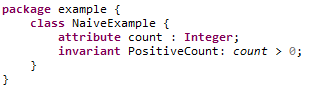
\includegraphics[width=5.0in]{NaiveExample.png}
	\end{center}
	\vspace{-10pt}
	\caption{Naive Example}
	\label{fig:NaiveExample}
	\vspace{-10pt}
\end{figure}

Our running example considers the very simple class constraint shown using OCLinEcore\cite{OCLinEcore} in Fig~\ref{fig:NaiveExample}.

The \verb|NaiveExample| class contains an \emph{Integer} attribute named \verb|count| and an invariant to require a positive value.

It would seem self evident that the invariant is 2-valued corresponding to satisfied/not-satisfied, but it is not. There are two crash hazards.

\subsection{Hazards}

If the host model is served by a cloud network or database, there is a possibility that the \emph{PropertyCallExp} access to \verb|count| may fail with some form of network error. This error is treated as \verb|invalid| by OCL and consequently the evaluation of the constraint yields an \verb|invalid| result. As noted above, this rather pedantic but catastrophic concern is resolved by a strict any-crash-always-crashes philosophy.

Fig~\ref{fig:NaiveExample} also shows the OCLinEcore editor's hover text to
reveal the underlying \emph{Property} declaration with a fully qualified name \verb|example::NaiveExample::count|, primitive type \verb|Integer| and multiplicity \verb|[?]|. The optional multiplicity allows the value of \verb|count| to be \verb|null|. In Ecore \cite{EMF}, where the emphasis is on simple default construction of Java objects, the default multiplicity lower bound for all objects is 0. Consequently this is the OCLinEcore default and so a widespread practice. In contrast for UML, the lower bound multiplicity default is unity so that a \verb|null| is only permitted after an explicit user action. Either way, a valid \emph{Property} may specify that \verb|null| is an acceptable value. The \verb|null| value violates the strict precondition of the comparison operation. It crashes the invariant and disappoints the user hoping for a 2-valued outcome.

We require our tooling to support elimination of this not-2-valued hazard by diagnosing that the required non-null/non-invalid input of the comparison operator is \emph{MayBeNull}.

\subsection{Fixes}

The user may easily fix the problem by correcting the optional \verb|[?]| multiplicity to the non-optional \verb|[1]|. Alternatively, if a \verb|null| value is a required aspect of the design, the user may correct the invariant as shown in Fig~\ref{fig:FixedExample}.

\begin{figure}
	\vspace{-10pt}
	\begin{center}
		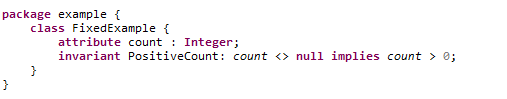
\includegraphics[width=6.0in]{FixedExample.png}
	\end{center}
	\vspace{-10pt}
	\caption{Fixed Example}
	\label{fig:FixedExample}
	\vspace{-10pt}
\end{figure}

The \verb|implies| operation guards the comparison preventing the crash, but naively the tooling will continue to diagnose the hazard unless the tooling understands the program control flow consequences of the sequentially-strict \verb|implies| operation.

\section{Program Analysis}\label{Program Analysis}

Our running example shows that even simple OCL code can have a problem that can be fixed. We now introduce an analysis to alert the user for the need for fixes and confirm that sufficient fixes have been applied to guarantee that no undesirable crashes occur and that all desirable crashes always crash. We first review the conventional run-time evaluation of our example OCL expression.

\begin{verbatim}
    self.count <> null implies self.count > 0
\end{verbatim}

\subsection{Simple Evaluation}\label{Simple Evaluation}

The OCL specification defines the Abstract Syntax of OCL expressions. Fig~\ref{fig:FixedExampleAST} shows the Pivot-based Eclipse OCL AST of the fixed example invariant using a UML Object Diagram-like exposition of the XML serialization. (Solid lines and diamonds for compositions, dashed lines for references.)

\begin{figure}
	\vspace{-10pt}
	\begin{center}
		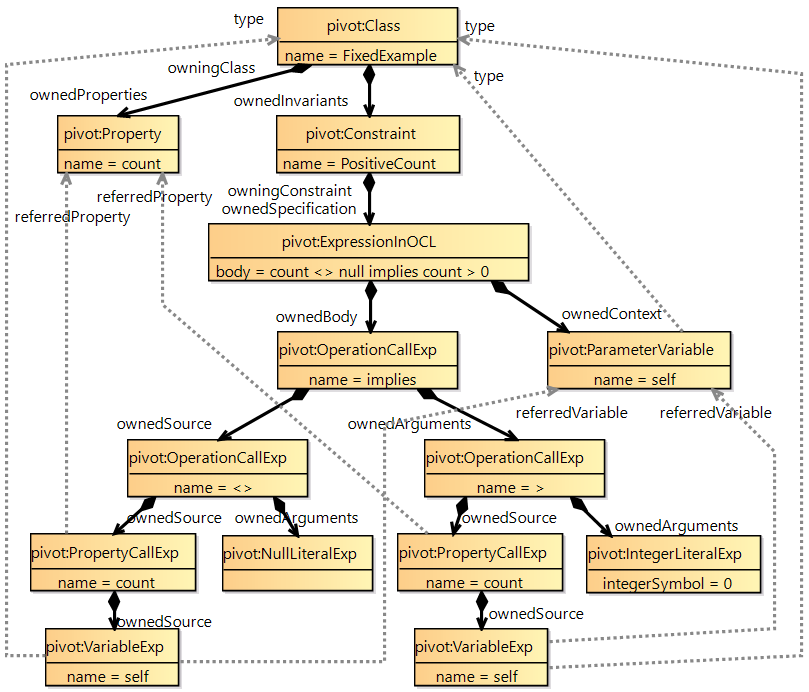
\includegraphics[width=4.5in]{FixedExampleAST.png}
	\end{center}
	\vspace{-10pt}
	\caption{Fixed Example Abstract Syntax Tree}
	\label{fig:FixedExampleAST}
	\vspace{-10pt}
\end{figure}

The top of the diagram shows the \verb|FixedExample| \emph{Class}, \verb|count| \emph{Property} and \verb|PositiveCount| \emph{Constraint} metamodel elements. The \emph{Constraint} is realized by an \emph{ExpressionInOCL} with a \verb|self| \emph{ParameterVariable} and the \emph{ownedBody} OCL expression tree with an \verb|implies| \emph{OperationCallExp} at its root\footnote{The \emph{referredOperation} links to the Standard Library model are omitted}.

The \emph{ownedSource} sub-tree comprises another \emph{OperationCallExp} for the \verb|<>| operation with further sub-trees comprising a \emph{PropertyCallExp} to evaluate the \verb|count| property upon the result of the \emph{VariableExp} that accesses the \verb|self| \emph{ParameterVariable}. The second sub-tree comprises a \emph{NullLiteralExp} that evaluates to the \verb|null| value.

The \emph{ownedArguments} sub-tree of the \verb|implies| comprises a very similar subtree to again evaluate \verb|self.count| but to use a \verb|>| operation to compare against the \verb|0| \emph{IntegerLiteralExp}.

At run-time this constraint may be used to confirm the well-formedness of each element of a user model. Each instance of \verb|FixedExample| is bound in turn to the \verb|self| \emph{ParameterVariable} and then the \emph{ownedBody} is evaluated by bottom up tree traversal with each descendant returning a result to its ancestor.

Execution therefore starts at the bottom left as a \emph{VariableExp} accesses the \verb|self| value and passes its value as the \emph{ownedSource} for its parent \emph{PropertyCallExp} that accesses the \verb|count| slot and passes it as the \emph{ownedSource} of the \verb|<>|. The depth first traversal continues by providing \verb|null| as the \emph{ownedArguments} input of the \verb|<>| from the \emph{NullLiteralExp}. With both inputs computed, the \verb|<>| can pass its result to as  \emph{ownedSource} for the \verb|implies|, which once a similar traversal has computed its \emph{ownedArguments} input can return the overall result to the \emph{ExpressionInOCL}.

\subsection{Precondition Evaluation}\label{Precondition Evaluation}

In OCL, operations such as \verb|>| are strict requiring all inputs to be evaluated and to be non-invalid before execution. Whether operations also require non-null inputs is determined by the \verb|[?]| or \verb|[1]| multiplicity of each operation parameter. The specification wording can be formalized by preconditions.

\begin{verbatim}
    operation Integer::>(arg : Integer[1]) : Boolean {
        precondition: not self.oclIsInvalid();
        precondition: not arg.oclIsInvalid();
        precondition: not self.oclIsUndefined();
        precondition: not arg.oclIsUndefined();
        precondition: self.oclIsKindOf(Integer);
        precondition: arg.oclIsKindOf(Integer);
    }
\end{verbatim}

A full evaluation should validate these and other preconditions by evaluating them. Eclipse OCL~\cite{Eclipse-OCL} never executes preconditions. USE~\cite{USE} can do so when requested.

The conventional use of the OCL well formedness rules supports a static analysis that ensures that all input values are type compatible. Here we are concerned with a more extensive  static analysis to ensure that all preconditions are satisfied. The static analysis occurs at edit/compile-time making evaluation at run-time redundant.

\subsection{Symbolic Evaluation}\label{Symbolic Evaluation}

%In OCL,the logical operations such as \verb|implies| are not-strict in order to allow a fortuitous value for one input to obviate the computation of another which may therefore be permitted to be \verb|null| or \verb|invalid|. For \verb|implies|, if the first input is \verb|false|, the value of the second input is ignored,

%\begin{verbatim}
%    operation Boolean::implies(arg : Boolean) : Boolean {
%        precondition: not self.oclIsInvalid();
%        precondition: not self.oclIsUndefined();
%        precondition: self.oclIsKindOf(Boolean);
%        precondition: self = false or not arg.oclIsInvalid();
 %       precondition: self = false or not arg.oclIsUndefined();
 %       precondition: self = false or arg.oclIsKindOf(Integer);
%        body: not self or arg;
%    }
%\end{verbatim}

At edit/compile-time we have no actual instances, rather we need to prove that for all possible instances the result will be either 2-valued or a desirable crash. With our revision to strict semantics for everything except for the sequentially-strict logical operations we `just' need to prove that no undesirable crash can occur.

For our example, we have intuitively identified that \verb|self.count > 0| may crash for \verb|invalid| or \verb|null| values of \verb|count|. More rationally, the \verb|self| object is not \verb|invalid| and instance slots cannot contain \verb|invalid| values, so an \verb|invalid| value is only possible as a consequence of a database/network failure. This would be a desirable crash. However the instance slot can contain a \verb|null| value. The \verb|self.count <> null| guard uses \verb|implies| to protect against this \verb|null| value. Confirming this protection requires a \verb|false| value for the \verb|<>| output, enabling us to deduce that the inputs are different.
%Since \verb|count| is accessed from an instance slot, a desirable crash may occur from a database/network failure. An undesirable crash can occur for a \verb|null| or \verb|invalid| value. Slots cannot have \verb|invalid| values so only the \verb|null| value permitted by the multiplicity lower bound needs to be eliminated. The \verb|implies| guard idiom ensures that any crash while evaluating its second argument is ignored if the first argument evaluates to \verb|false|. The guard is \verb|false| when the \verb|<>| evaluates to \verb|false| which requires the inputs to differ; \verb|x| to differ from \verb|null|.

This achieves what we want, but it has required us to deduce properties of the \verb|<>| inputs from its output. This is a reverse evaluation that requires distinct implementation programming and which scales badly since only single input monotonic operations support useful deduction of an input from a known output.

We can avoid reverse flow deductions by instead hypothesizing that an undesirable crash can occur and demonstrate that forward evaluation leads to a contradiction. For our example, we consider the hypothesis

\begin{center}
	\begin{tabular}{c c}
		when: & self.count <> null \\
		execution is attempted for: & self.count > 0 \\
	\end{tabular}
\end{center}

This evaluation can be performed by a symbolic evaluator that elaborates the standard evaluator to use a symbolic value wherever a constant value is not known.

\subsection{Boolean Symbolic Evaluation}

For simple invariants it is sufficient for the \emph{SymbolicValue} to be a tuple maintaining the following information for our partial knowledge:
\begin{itemize}
	\item Value Type : Type[1]
	\item MayBeInvalid : Boolean[1]
	\item MayBeNull : Boolean[1]
\end{itemize}

The symbolic nullity state requires only two \emph{MayBeNull}, \emph{MayNotBeNull} values since the third \emph{IsNull} state uses the constant literal value of type \emph{OclVoid}.

The symbolic careless invalidity state requires only two \emph{MayBeInvalid}, \emph{MayNotBeInvalid} values since the third \emph{IsInvalid} state would be a deliberate and so desirable crash that bypasses our careless invalidity analysis.

For our example:

\begin{verbatim}
    self.count <> null implies self.count > 0
\end{verbatim}

The symbolic evaluation needs to confirm that no undesirable crash can occur for the \verb|>| \emph{OperationCallExp} in \verb|self.count > 0|.

\subsubsection{Base Symbolic Evaluation}

An overall symbolic evaluation of an invariant uses the initial symbolic value.
\begin{center}
	\begin{tabular}{|c||c|c||c|}
		\hline
		Symbolic Variable & Value Type & MayBeInvalid & MayBeNull \\
		\hline
		self & FixedExample & false & false \\
		\hline
	\end{tabular}
\end{center}
 and all other constraints and preconditions
\begin{center}
	\begin{tabular}{|c|c||c|}
		\hline
		AST element & AST Type & Precondition \\
		\hline
		\hline
		self & ParameterVariable & not self.oclIsInvalid() \\
		&& not self.oclIsUndefined() \\
		&& self.oclIsKindOf(FixedExample) \\
 		\hline
		self & VariableExp & \\
 		\hline
		null & NullLiteralExp & \\
 		\hline
		0 & IntegerLiteralExp & \\
		\hline
		self.count & PropertyCallExp & not source.oclIsInvalid() \\
		&& not source.oclIsUndefined() \\
		&& source.oclIsKindOf(FixedExample) \\
 		\hline
		self.count & OperationCallExp & not source.oclIsInvalid() \\
		<> && not arg.oclIsInvalid() \\
		null && not source.oclIsUndefined() \\
		&& not arg.oclIsUndefined() \\
		&& source.oclIsKindOf(Integer) \\
		&& arg.oclIsKindOf(Integer) \\
 		\hline
        self.count & OperationCallExp & not source.oclIsInvalid() \\
		> && not arg.oclIsInvalid() \\
		0 && not source.oclIsUndefined() \\
		&& not arg.oclIsUndefined() \\
		&& source.oclIsKindOf(Integer) \\
		&& arg.oclIsKindOf(Integer) \\
 		\hline
        self.count <> null & OperationCallExp & not source.oclIsInvalid() \\
		implies && not arg.oclIsInvalid() \\
		self.count > 0 && not source.oclIsUndefined() \\
		&& not arg.oclIsUndefined() \\
		&& source.oclIsKindOf(Boolean) \\
		&& arg.oclIsKindOf(Boolean) \\
		\hline
	\end{tabular}
\end{center}

giving the symbolic values of each AST node as

\begin{center}
	\begin{tabular}{|c||c|c|c|}
		\hline
		AST element & Value Type & MayBeInvalid & MayBeNull \\
		\hline
		\hline
		self & FixedExample & false & false \\
		\hline
		self.count & Integer & false & true\\
		\hline
		null & OclVoid & false & true \\ 
		\hline
		self.count <> null & Boolean & false & false \\
		\hline
		0 & Integer & false & false \\
		\hline
		self.count > 0 & Boolean & true & false \\
		\hline
		self.count <> null & Boolean & true & false \\
		implies self.count > 0 & & & \\
		\hline
	\end{tabular}
\end{center}

Five of the six \verb|>| preconditions are satisfied by the symbolic values.

The sixth, \verb|not source.oclIsUndefined()| might not be satisfied since, for its \verb|self.count| source, \emph{MayBeNull} is \verb|true| and propagates as \emph{MayBeInvalid} after the comparison.

\subsubsection{Hypothesized Symbolic Evaluation}

We can establish that the sixth precondition is satisfied by showing that the hypothesis that a \emph{null} value of the \verb|self.count| source can be used leads to a contradiction. 

We bind an additional non-symbolic value \verb|null| as the symbolic value of \verb|self.count|.

\begin{center}
	\begin{tabular}{|c||c|c||c|}
		\hline
		Symbolic Variable & Value Type & MayBeInvalid & MayBeNull \\
		\hline
		self.count & OclVoid & false & true \\
		\hline
	\end{tabular}
\end{center} 

We impose additional preconditions on the short-circuit and if-then-else ancestors of the hypothesized value to ensure that the control path that evaluates the hypothesized value is used.

\begin{center}
	\begin{tabular}{|c|c||c|}
		\hline
		AST element & AST Type & Constraint \\
		\hline
		\hline
        self.count <> null & OperationCallExp & source = true \\
		implies self.count > 0 && \\
		\hline
	\end{tabular}
\end{center}

Re-evaluating the symbolic values of each AST node for the new known values and checking all constraints finds the required contradiction. \verb|self.count <> null| now evaluates to \verb|false| contradicting the new precondition that the \verb|self.count <> null| source is \verb|true|.

\subsubsection{Intuition}
 
Our running example is very simple, closely emulating the simplest of guard idioms that most programmers have used many times. The solution is therefore pretty intuitive.

Laboriously working through the example as symbolic values, constraints, hypothesis and contradiction demonstrates how the magic of intuition and reverse evaluation is replaced by predictable rigor that can scale to non-trivial problems.

Boolean Symbolic Evaluation is sufficient to cope with the complexities of unsafe usage of \verb|null| or \verb|invalid|.

\subsection{Real Symbolic Evaluation}

Although OCL is not often used for floating point calculations, OCL provides a \emph{Real} type for which division by zero has an undesirable crash hazard.

\begin{verbatim}
    operation Real::/(den : Real) : Real {
        precondition: den <> 0;
    }
\end{verbatim}

The edit/compile-time analysis should therefore diagnose the rare divide-by-zero hazards.

For the simple case, it is sufficient for a \emph{SymbolicRealValue} to maintain a \emph{MayBeZero} state so that the typical

\begin{verbatim}
    if den <> 0 then num / den else ... endif
\end{verbatim}

detects that the divide-by-zero case has been avoided and that the programmer has taken responsibility for solving the problem.

For the general case, it is unlikely that a symbolic analysis can adequately understand non-trivial floating point operations and so the programmer will be forced to adopt the simple-case guard.

\subsection{Integer and Collection Symbolic Evaluation}

In addition to an \emph{Integer} variant of the rare divide-by-zero hazard, a much more serious hazard arises from a bad index for e.g.

\begin{verbatim}
    aSequence->at(badIndex)
\end{verbatim}

\begin{verbatim}
    operation Sequence<T>::at(i : Integer) : T {
        precondition: i > 0;
        precondition: i <= self->size();
    }
\end{verbatim}

A \emph{SymbolicIntegerValue} needs to track any knowledge regarding the \emph{Maximum} or \emph{Minimum} possible values both as absolute or relative to the \verb|size()| of a base \emph{SymbolicCollectionValue}. 

\begin{itemize}
	\item Actual Type : Type[1]
	\item MayBeInvalid : Boolean[1]
	\item MayBeNull : Boolean[1]
    \item Maximum : Integer[?]
	\item Minimum : Integer[?]
    \item MaximumBase : SymbolicCollectionValue[?]
    \item MinimumBase : SymbolicCollectionValue[?]
\end{itemize}  

The symbolic evaluation of all collection operations needs to relate the output symbolic value to the input so that for e.g. \verb|Sequence::append|, the minimum and maximum output size is one larger than the input size. But for e.g.
\verb|OrderedSet::append|, only the maximum output size increases.

%The OCL specification provides the preconditions for many of the operations, but omits many others. Thus \verb|Sequence->first| omits an explicit \verb|size() > 0| precondition leaving the \verb|result = self->at(i)| postcondition to provide the undesirable crash from the nested precondition.

\subsection{Content Symbolic Evaluation}

In addition to tracking the sizes of collections it is also necessary to track known content of collections so that an \verb|includes| guard or \verb|including| action can satisfy the validity requirements of a subsequent \verb|any| iteration.

%The relevant guards and actions may be present ab initio, or may be added in order to satisfy that validity analysis. It is anticipated that most additional guards needed by the validity analysis will be genuine bug fixes rather than bloat just to placate tooling. 

\section{Corollaries}\label{Corollaries}

Our validity analysis has the goal of guaranteeing that no precondition ever fails. This changes the utility and capabilities of the tooling.

\subsection{Preconditions}

Without the analysis, a precondition is an additional expression that may cause a crash if evaluated at run-time on actual model values. Since the precondition often just anticipates a crash that would occur anyway, the utility of a precondition is limited to improving the diagnostic that accompanies the crash.

With the analysis, executing preconditions at run-time is redundant. The symbolic execution, at edit/compile-time, on all possible symbolic model values, guarantees that the precondition is satisfied.

Preconditions become an important part of the design and are exploited and checked at edit/compile-time. A too-weak precondition will be diagnosed by a crash hazard within the operation declaring the precondition. A too-strong precondition will be diagnosed by a crash hazard when the operation declaring the precondition is invoked.

%Once preconditions are used, it becomes clear that the OCL specification has significant omissions.  For instance the \verb|Sequence::first()| operation requires more than just a \verb|result = self->at(1)| postcondition. There should also be an explicit rather than transitive \verb|self->notEmpty()| precondition.

\subsection{Bodyconditions and BodyExpressions}

The Object Constraint Language is actually an expression language so that the functionality of an \emph{Operation} or \emph{Property} is characterized by a bodyexpression for the respective \emph{ownedBody} or \emph{ownedDefaultValue}. UML only supports constraints and so the \verb|result = bodyexpression| idiom reformulates the arbitrarily-typed bodyexpression as the Boolean-typed \emph{Constraint}. The UML exposition is indistinguishable from a postcondition.

When specifying OCL, the use of a bodyexpression is desirable when the expression represents a sensible implementation that can be used as is.

\subsection{Postconditions}

For an operation such as \verb|sort()| a postcondition is appropriate to specify the generic characteristics of a bubble or quick sort without imposing any particular implementation. 

In addition to the obvious \verb|result = ...| to specify the final result, it is also necessary to provide postconditions for each of the properties of the \emph{SymbolicCollectionValue} such as 
\verb|result->size() = self->size() + 1|.

%Similarly \verb|Sequence::including(object:T)| operation requires more than just a postcondition \verb|result = self.append(object)|. There should also be an explicit rather than transitive \verb|self->size() = self@pre->size()+1| postcondition. And once we start to rectify pre and post conditions omissions;, we notice errors in those that are present. The specified postcondition has two errors; it should be \verb|result = self@pre->append(object)| and would be simpler and more useful as a body expression \verb|self->append(object)|. Pedantically we should also provide a nothing-else-changes framing condition, but with OCL inherently immutable perhaps this can be left as read.

Postconditions are never executed by Eclipse OCL. Their execution may be requested in USE. When executed at run-time, they require execution overheads for no benefit, until one fails, at which point a crash must be handled.

Once postconditions form part of the edit/compile-time analysis many too-weak/too-strong problems may be uncovered in the same way as for preconditions. For library operations at least, a new occasional build-time test could animate each operation with a diverse suite of input values that check the postconditions. For model operations, a similar opportunity exists but work on automated test model generation has revealed challenges. 


%They could be but will burn time for the almost all cases that are problem free. Once they participate in the validity analysis, their utility will be conformed by usage. On an operation by operation basis, it could be tractable to auto-generate a diverse suite of library operation calls so that the postconditions can be extensively exercised at build-time.

%Invariants are currently executed by a dedicated validation tool, or validation pass of some more general modelling tool. The validity analysis can use invariants as additional opportunities to contract a may-be-xx hypothesis. 

\subsection{Assertions}

The new validity analysis benefits from its metamodel focus, but it is never going to be as powerful as a mathematical proof tool and even such specialized tools are unable to prove everything. It is therefore inevitable that a pessimistic validity analysis will have false positives diagnosing non-hazards. 

The user will have to provide assistance. An additional invariant or a more explicit guard may often solve the problem. For the harder cases it may be necessary to add an assertion capability.

\begin{verbatim}
    OclAny::oclAssert(constraint : Lambda(T) : Boolean[1],
        justification : String[1]) : OclAny = self
\end{verbatim}

The assertion returns its source as its result and asserts that the \verb|constraint| is true for the result\footnote{The \emph{Lambda} type is the consequence of modeling the passing of OCL expressions to e.g. iteration bodies.}. The \verb|constraint| may link to a possibly formal proof of the \verb|constraint| facilitating a QA review of the ad hoc assertions.

The challenge is therefore to make the program flow analysis powerful enough to reduce the number of false positives to a level where the extra user effort to resolve the hazards is more than repaid by the benefits of no crashes. %to provide extra invariants, guards or assertions is small enough in comparison with the benefit of the guarantee that there are no undesirable crashes so that invariants are 2-valued and model transformations crash comprehensively.

In many cases, the need for an assertion may alert the user to an unjustified optimism as to the true characteristics of all possible models.

\subsection{Static Single Assignment}

Symbolic evaluation in OCL is much simpler than in many other languages since OCL is side effect-free, consequently any Common Sub-Expression \cite{DragonBook} is immutable and has the same (symbolic) value wherever used. In other languages it may be necessary to refactor to construct a Static Single Assignment representation in which each variable has only a single value. For OCL, all terms are inherently in SSA form.

\subsection{Multiple/Cascade Invariants}

The constraints for a non-trivial class often comprise some simple obvious constraints and increasingly complicated constraints that depend on the simpler ones.

If each constraint is written in its minimal form and each constraint is checked individually, the tooling is liable to accompany the diagnosis of a simple constraint failure by gratuitous crash diagnoses from the more complicated constraints.

Conversely, if each constraint is written in its maximal form, the duplication of each simple constraint makes the more complicated constraint hard to read and so leads to maintenance difficulties.

%The bloat of maximal form could be eliminated by refactoring simpler constraints as Boolean-valued operations that can be used as predicates in the complex constraints. This could be supported automatically if named invariants were automatically recognized as definitions of Boolean-valued operations.

%Neither UML nor OCL specifications provide any style guidance for this.

Once we use symbolic evaluation and associate a distinct symbolic value with each distinct AST element, the dilemma goes away. The multiple constraints are part of a logical conjunction for which common sub-expression elimination removes duplicates. Symbolic evaluation observes expression precedence to only traverse credible paths once. Only the first failure in the depth first traversal will be diagnosed.

%The style guidance can therefore be to write constraints in minimal form and to sequence many simple constraints in whatever order is easiest for a human to understand. The tooling doesn't care about the order but humans can most easily understand execute constraints in order.

\subsection{Exceptions}

Our validity analysis guarantees that no undesirable crashes occur, and that desirable crashes always crash. For the benefit of Operating System level OCL that needs to handle a genuine crash, the ability to use \verb|OclAny::oclIsInvalid()| to catch a crash could be enhanced by a \verb|OclAny::oclAsException()| method to unpack the \verb|invalid| singleton into a new \emph{Exception} class instance for comprehensive handling.

\section{Current Status and Further Work}\label{Current Status and Further Work}

This phase of work was initially driven by the challenges of faithfully implementing undesirable crashes for a QVTc/QVTr Java code generator~\cite{Eclipse-QVTd}. The inconveniences of uncrashing logical operations spiral once the logical operations define complex relation guards; an unmatching capability is required. Since the awkwardness of the implementation corresponds quite closely to surprising behavior for the user, it is much more appropriate to push back and alert the user to the hazards and so avoid generating any of the difficult code. For model transformation, the no undesirable crashes, all-crashes-always-crash policy is better, simpler and faster.

The work continued the null-safe navigation work \cite{Safe OCL} which initially required almost all navigation operators to be changed to their safe counterparts; a widespread effort for no real benefit. Extending the null-safe declarations to support null-free collection reduced the changes to genuine hazards. However limited heuristic program control flow analysis meant that only simple guards were recognized as avoiding the hazard.

The new work expands from just null hazards to all precondition failures with a much more comprehensive program flow analysis to propagate, for instance, a known symbol collection size or content to discount a hazard.

The initial approach of deducing the values of variables backwards from the point at which a guard provides extra knowledge gave way to a forward evaluation of all relevant constraints to contradict \emph{IsXxx} hypotheses at each potential hazard.

Once the focus shifts to a forwards symbolic evaluation, it is then just necessary to improve the formulation of the library operations.


%Preconditions are now elevated from the cosmetic status of syntax-checked comments to the declarations of undesirable crash hazards that edit/compile-time analysis must diagnose so that the user can eliminate them.

%Bodyconditions/body expressions can be preferred over postconditions when the a sensible constructive algorithm for the result is provided.

%Postconditions are appropriate for operations such as sort() for which a declaration of the effect is considerably simpler than an optimized implementation such as quiksort. Postconditions are necessary to specify a derived characteristics of the result such as the size or known content of a collection result.

%Preconditions are currently not-executed since when correctly coded they just burn time predicting the crash that will occur anyway. They can now participate in the validity analysis for execution at edit/compile-time. A too-narrow precondition will cause problems for a user when invocations are unexpectedly rejected. A too-broad precondition should be diagnosed as the validity analysis fails to conform the safety of the precondition.

%\subsection{Desirable Crashes Revisited}

%Once the problems with undesirable rashes are resolved by analysis, we need to ensure that desirable crashes crash properly. If the desirable crash is guardable, the desirable crash should not occur. Currently in:

%\begin{verbatim}
%	functionReturningCrash() and functionReturningFalse()
%\end{verbatim}

%most implementations will first invoke \verb|functionReturningCrash| before \verb|functionReturningFalse| so that anyone observing execution, perhaps using a debugger, will see the crash happening and be confused that no desirable crash actually occurs because \verb|functionReturningFalse| guards it.

%We can use the validity analysis to ensure that a desirable crash is either avoided or propagated but never hidden. If the mayBeNullOrInvalid hypothesis cannot be contradicted for both arguments, the terms can be reordered to only crash on the second term allowing a non-crashing first term to consistently guard the second. If the mayBeNullOrInvalid hypothesis cannot be contradicted for either argument, the hazard must be diagnosed and the user may be recommended to put at least the second argument into a let-variable to ensure that it is not guarded. The foregoing makes only a minor change to the concurrent/commutativity of the \verb|and| arguments; The second argument must be proved to be not-null and not-invalid. This is a much smaller semantic change than the redefinition of \verb|and| to support the conventional sequential execution and consequent simple short-circuiting of more familiar languages.

\section{Related Work}\label{Related Work}

Preconditions and postconditions are an essential part of design by contract endorsed by the OCL specification~\cite{OCL-2.4}, but because they are not much used in practice, these deficiencies in the OCL specification have not been reported. The USE tool~\cite{USE} is able to execute preconditions and postconditions at run-time. Eclipse OCL~\cite{Eclipse-OCL} never executes them.

The inadequacy of preconditions and postconditions has been highlighted by the proposals to add support for framing conditions \cite{Framing} that simplistically assert that nothing else changes. It is not clear that framing conditions are necessary for OCL since the prohibition on side-effects ensures nothing changes that isn't mentioned in a postcondition.  

Work on automated test model generation \cite{Brucker},\cite{Francisco},\cite{Gogolla} produces suites of test models that can be animated. The preconditions can guide the production of good models and motivate the production of bad models.

Tools such as EMFtoCSP \cite{EMFtoCSP} and UMLtoCSP establish metamodel consistency by searching for models that demonstrate that all metamodel constraints can be satisfied. An inadequate metamodel is detected if a particular class or constraint is dead with respect to all models searched. The constraints are translated from OCL to a CSP solver where they are repetitively evaluated for candidate models. 

These usages rely on converting the (UML) metamodel and OCL constraints into the language of a CSP or SAT solver where searches/syntheses proceed. The precondition is assumed to be internally good and the corollaries are assessed.

In this work, each precondition is proved to be internally good without needing to synthesize any models. Whether the precondition contributes to a usable system is not relevant. We just guarantee that no precondition can ever fail and so remove an impediment to both normal and automated search usage.

%\subsection{Summary of Changes}\label{Summary of Changes}

%We have previously advocated introducing an \verb|error| value to distinguishing the desirable (really strict) and undesirable (somewhat strict) crash forms of \verb|invalid|. However this creep evolves the Boolean type to 5-value, which is unlikely to meet approval from those keen to see a 2-value Boolean. 

%The new analysis enables the troublesome not-strict \verb|crash and false| case to be detected and so eliminated at edit/compile-time. For an undesirable or unwanted crash, the user can refactor as \verb|false and crash|. For a desirable crash, the user can remove the trailing guard. With the troublesome case eliminated, the run-time needs no irregular strictness treatment for the logical operators, just a short-circuit capability.

%The library specification requires a rework to correct existing constraints and provide the more comprehensive constraints necessary for symbolic evaluation.

%String operations that return \verb|invalid| for inadequate lexical content should be redefined to return \verb|null|.

%A new \verb|oclAssert| library operation is required to allow the user to help with complex expressions for which symbolic evaluation fails to find known contradictions.

%A new \verb|oclAsException| library operation is required to support handling of desirable crashes for Operating System level OCL programming.

\section{Conclusions}\label{Conclusions}

We have identified the inadequate consideration of crashes as a contribution to the disappointment of many OCL users that constraints are not 2-valued.

We have distinguished between catastrophic desirable crashes and careless undesirable crashes from precondition failures.

We have introduced a compile-time analysis to detect and so guarantee that desirable crashes always crash and that undesirable crashes never occur.

We can look forward to common programming errors such as off-by-one ordered collection index crashes being avoided and so find that constraints are indeed the 2-value construct that users expect.

The prototype implementation within Eclipse OCL shows promise but has revealed how much more can be done.


%
% ---- Bibliography ----
%
\begin{thebibliography}{}

\bibitem{DragonBook}
Aho, A., Sethi, R., Ullman, J.: Compilers, Principles, Techniques and Tools, Addison Wesley, 1986

\bibitem{Brucker}
Brucker, A., Krieger, M., Longuet, D., Wolff, B.: A Specification-based Test Case Generation Method for UML. 10th International Workshop on OCL and Textual Modeling, October, 2010, Oslo, Norway.
\url{https://modeling-languages.com/events/OCLWorkshop2010/submissions/ocl10\_submission\_7.pdf}

\bibitem{Francisco}
Francisco, M., Castro, L.: Automatic Generation of Test Models and Propertiesfrom UML Models with OCL Constraints. 12th International Workshop on OCL and Textual Modeling, September, 2010, Innsbruck, Austria.\\
\url{https://st.inf.tu-dresden.de/OCL2012/preproceedings/07.pdf}

\bibitem{Gogolla}
Gogolla, M., Burgue\~no, L., Vallecillo, A.: EMFtoCSP: A Tool for the Model Finding and Model Completion with USE. 18th International Workshop on OCL and Textual Modeling. Copenhagen, Denmark, October 14, 2018.
\url{https://ceur-ws.org/Vol-2245/ocl_paper_9.pdf}

\bibitem{EMFtoCSP}
Gonz\`alez, C., B\~uttner, F., Claris\'o, R., Cabot, J.: EMFtoCSP: A Tool for the Lightweight Verification of EMF Models. Formal Methods in Software Engineering: Rigorous and Agile Approaches (FormSERA), Jun 2012, Zurich, Switzerland. hal-00688039
\url{https://hal.inria.fr/file/index/docid/688039/filename/emftocsp.pdf}

\bibitem{Framing}
Przigoda, N., Filho, J., Niemann, P., Wille, R.: Frame Conditions in Symbolic Representations of UML/OCL Models. 2016 ACM/IEEE International Conference on Formal Methods and Models for System Design (MEMOCODE), 2016, pp. 65-70, doi: 10.1109/MEMCOD.2016.7797747.\\
\url{https://iic.jku.at/files/eda/
2016\_memocode\_frame\_conditions\_symbolic\_representation.pdf}

\bibitem{EMF}
Steinberg, D., Budinsky, F., Paternostro, M., Merks, E.: EMF: Eclipse Modeling Framework. Addison-Wesley, Jun 2008

\bibitem{OCLreflections}
Willink, E.: Reflections on OCL 2. Journal of Object Technology. Vol.19, No. 3, 2020.\\ \url{https://dx.doi.org/10.5381/jot.2020.19.3.a17}

\bibitem{Safe OCL}
Willink, E.: Safe Navigation in OCL.
15th International Workshop on OCL and Textual Modeling, September 8, 2015, Ottawa, Canada.\\
\url{https://ocl2015.lri.fr/OCL\_2015\_paper\_1111\_1400.pdf}

\bibitem{OCL-2.4}
Object Constraint Language. Version 2.4., OMG Document Number: formal/2014-02-03, Object Management Group. February 2014,  \url{https://www.omg.org/spec/OCL/2.4}

\bibitem{QVT-1.3}
OMG. Meta Object Facility (MOF) 2.0 Query/View/Transformation Specification, Version 1.3.
OMG Document Number: ptc/16-06-03, June 2016.
\url{https://www.omg.org/spec/QVT/1.3}

\bibitem{UML-2.5}
OMG Unified Modeling Language (OMG UML), Version 2.5, {OMG Document Number}: formal/15-03-01, Object Management Group, March 2015,\\ \url{https://www.omg.org/spec/UML/2.5}

\bibitem{Eclipse-OCL}
Eclipse OCL Project.
\url{https://projects.eclipse.org/projects/modeling.mdt.ocl}

\bibitem{Eclipse-QVTd}
Eclipse QVT Declarative Project.\\
\url{https://projects.eclipse.org/projects/modeling.mmt.qvtd}

\bibitem{OCLinEcore}
OCLinEcore.
\url{https://wiki.eclipse.org/OCL/OCLinEcore}

\bibitem{USE}
USE, The UML-based Specification Environment. \\ \url{https://useocl.sourceforge.net/w/index.php/Main\_Page}

\end{thebibliography}
\end{document}
